\section{Theorie}
\label{sec:Theorie}

\subsection{Aufbau und Funktionsweise}
\label{sec:aufbau}

Der Aufbau des Geiger-Müller-Zählrohrs ist in \autoref{fig:querschnitt} dargestellt. Es besteht aus
einem Kathodenzylinder (Radius $R_\text{k}$) und einem mittig liegenden, axial verlaufenden
Anodendraht (Radius $R_\text{a}$) und wird mit einem Gasgemisch gefüllt.
\begin{figure}[H]
	\centering
	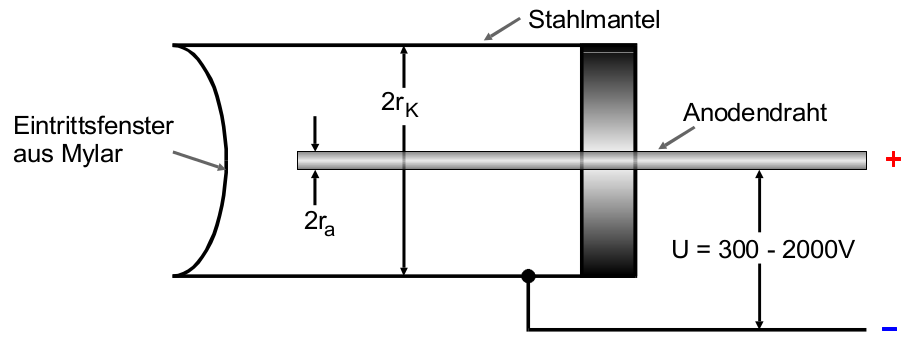
\includegraphics[width=0.8\textwidth]{content/aufbau.png}
	\caption{Querschnitt durch ein Endfenster-Zählrohr \cite{sample}}
	\label{fig:querschnitt}
\end{figure}
\noindent
Bei Anlegen einer Spannung $U$ verhält sich das Rohr wie ein zylindrischer Kondensator, woraus die 
radialsymetrische elektrische Feldstärke
\begin{equation}
	E = \frac{U}{r \ln(r_\text{k} / r_\text{a})}
	\label{eqn:elektrisches-feld}
\end{equation}
folgt.

\noindent
Es soll jetzt ein geladenes Teilchen, welches in das Zählrohrvolumen eindringt, betrachtet werden. Unter
der Annahme, dass es vollständig absorbiert wird, wird es sich durch den Gasraum bewegen, bis es seine 
Energie durch Ionisationen abgegeben hat. Dabei wird im Mittel eine Energie von $26\ \si{\eV}$ 
abgegeben \cite{detektoren}.
Die Teilchen, die wir hier betrachten, haben eine Energie in der Größenordnung $10^5\ \si{\eV}$, d.h. 
dass die Anzahl an Ionisierungen und der dabei freigesetzten Elektronen proportional zur Energie des 
einfallenden Teilchens sind.

\noindent
Dabei ist wichtig, dass die Vorgänge nach der ersten Ionisation im Zählrohr stark von der Spannung $U$ 
abhängen, der Zusammenhang ist in \autoref{fig:ionisationen-u} dargestellt.
\begin{figure}
	\centering
	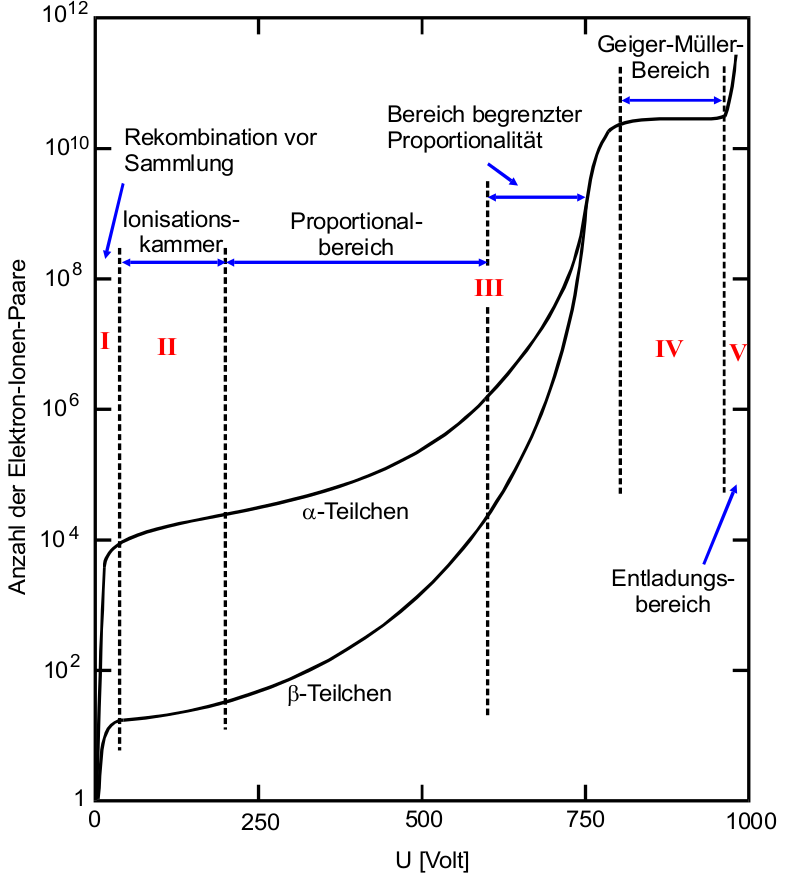
\includegraphics[width=0.6\textwidth]{content/ionisationen-u.png}
	\caption{Anzahl der erzeugten Elektron-Ionenpaare als Funktion der Spannung U bei einem
	Proportionalzählrohr (nach Kleinknecht, Detektoren für Teilchenstrahlen) \cite{sample}}
	\label{fig:ionisationen-u}
\end{figure}
Dabei sind einige Bereiche bei $U$ zu unterscheiden:
\begin{itemize}
	\item Für kleine Spannungen geht nur ein Teil der Ionisationselektronen zur Anode, der Rest geht 
		durch Rekombination verloren. (Entspricht Bereich \Romannum{1} in \autoref{fig:ionisationen-u})
	\item Bei höheren Spannungen (Bereich \Romannum{2}) 
		sinkt die Rekombinationswahrscheinlichkeit ab, sodass alle erzeugten Elektronen
		die Anode erreichen. Der Ionisationsstrom ist dabei proportional der Intensität und Energie
		der einfallenden Strahlung. Unter diesen Vorraussetzungen wird ein Gerät als Ionisationskammer
		bezeichnet, eignet sich jedoch nur bei hohen Strahlungsintensitäten.
\end{itemize}
